\chapter{Backoffice}
Il Backoffice è l'applicazione web che permette ai gestori degli impianti presenti su eServant di:
\begin{itemize}
    \item configurare i propri impianti, per ogni impianto gli eventi e per ogni evento i servizi disponibili
    \item monitorare real-time l'impianto analizzando i dati provenienti dai sensori IoT
    \item monitorare e analizzare offline le prestazioni del sistema/impianto dopo un evento o in un certo periodo
\end{itemize}

\begin{figure}[H]
    \centering  
    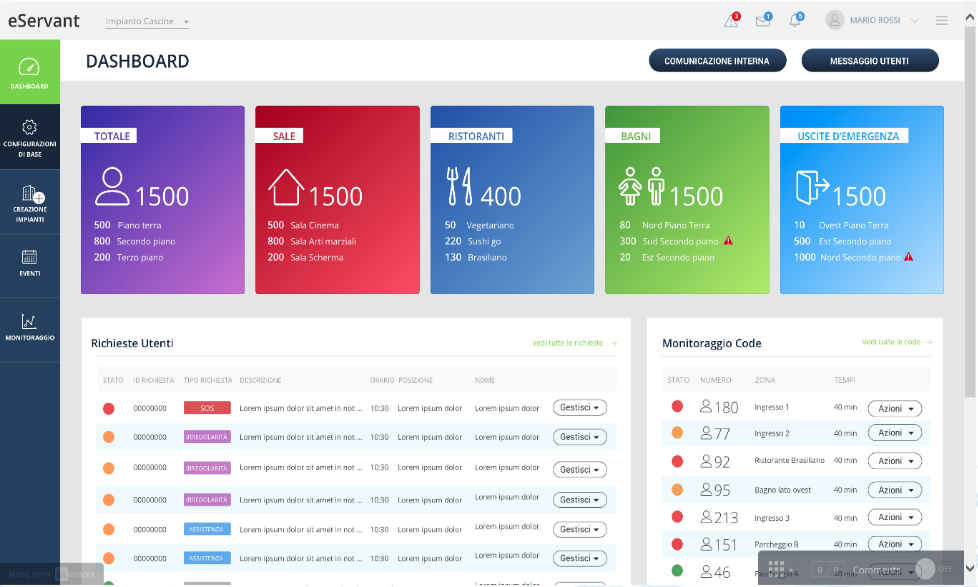
\includegraphics[scale=0.4]{img/cap3/backoffice}
\end{figure}

Il backoffice di eServant è stato realizzato con il framework Angular usando interamente Material Design come
sistema di progettazione dell'esperienza utente.
Material Design è un framework open source dell'azienda Google che aiuta i team a creare esperienze digitali
di alta qualità in breve tempo.

\section{Material Design}
Material Design mette a disposizione al team di sviluppo un set di componenti plagAndPlay solo da personalizzare
secondo il tema del brand utilizzatore.
Il principale vantaggio riscontrato è stata la velocità di sviluppo. Avendo nella maggior parte dei
casi dei componenti pronti all'uso ci ha permesso di concentrarsi sulla logica in Typescript invece che
sull'esperienza utente (non da sottovalutare).\\

I principali componenti messi a disposizione da Material Design di Google sono:

\begin{itemize}
    \item Componenti per i form
    \item Navigazione
    \item Layout
    \item Bottoni
    \item Popup
    \item Tabelle dati
\end{itemize}

Riporto un frammento di codice HTML usato nel backoffice di eServant ed il relativo effetto
nell'interfaccia utente.

\begin{lstlisting}[language=html]
<form class="newsform">
..
  <mat-form-field class="newsform__field">
    <input matInput placeholder="Titolo"">
  </mat-form-field>
..
</form>
\end{lstlisting}

\begin{figure}[H]
    \centering  
    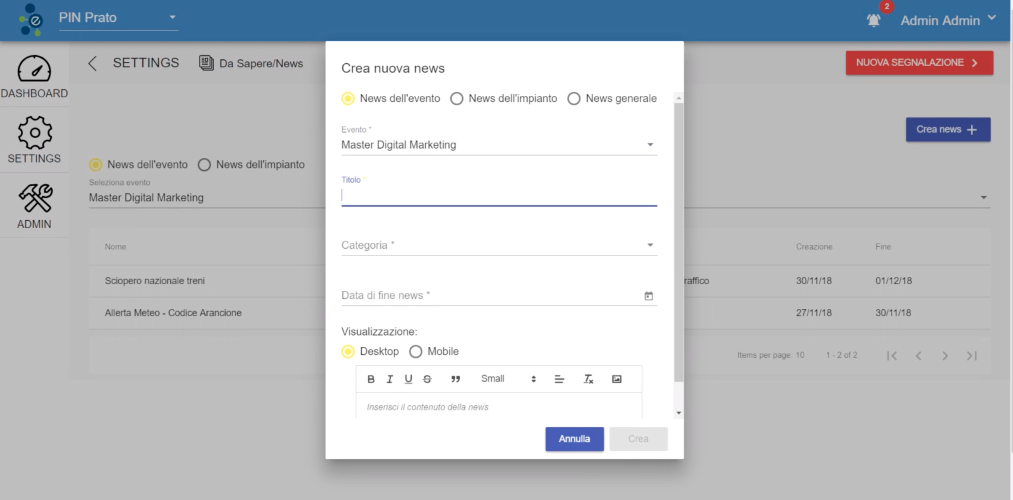
\includegraphics[scale=0.4]{img/cap3/backoffice-form}
\end{figure}

\section{BEM}
"There are only two hard problems in Computer Science: cache invalidation and naming things" cit. Phil Karlton

È noto che un'organizzazione corretta dei fogli di stile può aumentare significativamente la velocità
di sviluppo, il debug e l'implementazione di nuove feature. Purtroppo, molti codici CSS vengono
sviluppati senza alcuna convenzione di struttura o di nome. Ciò porta a una base di codice CSS 
non mantenibile a lungo termine.

L'approccio BEM cerca di garantire a tutti i partecipanti attuali e futuri allo sviluppo di un sito web
lavorino con un singolo base code e parlino la stessa lingua. 

BEM è l'acronimo di 
\begin{itemize}
\item Block
\item Element
\item Modifier
\end{itemize}

\begin{figure}[H]
    \centering  
    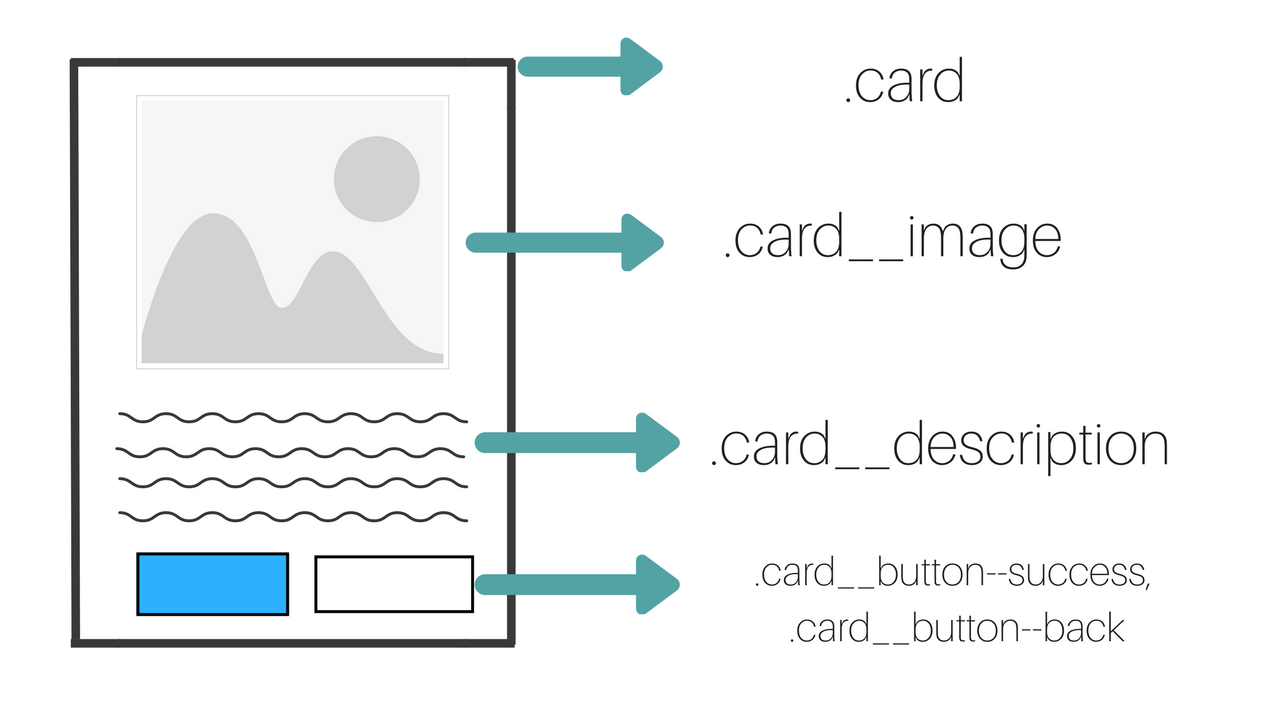
\includegraphics[scale=0.4]{img/cap3/bem}
\end{figure}

Analizziamo le classi CSS usate:

\begin{itemize}
    \item \textit{.card} è un \textbf{block}
    \item \textit{.card{\_}image} e  \textit{.card{\_}descriptor} sono \textbf{Element} di \textit{.card}
    \item \textit{.card{\_}image--success} e  \textit{.card{\_}descriptor--back} sono 
    \textbf{Modifier} di \textit{.card{\_}image}
\end{itemize}

Vediamo come è stato usato BEM nel caso specifico dell'header.

\begin{figure}[H]
    \centering  
    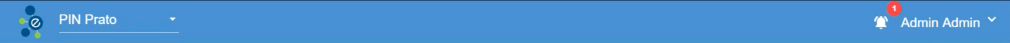
\includegraphics[scale=0.4]{img/cap3/header}
\end{figure}

\begin{lstlisting}[language=html]
<mat-toolbar class="header">
    <mat-toolbar-row>
        <img class="header__logo">
        <mat-select class="header__facilities">
            <mat-option *ngFor="let facility of facilities" [value]="facility.value">
            {{facility.display}}
            </mat-option>
        </mat-select>
        <mat-icon>alert</mat-icon>
        <div class="settings">
            <span class="settings__user">Admin</span>
            <mat-icon class="settings__icon settings__icon--closed">arrow-down</mat-icon>
        </div>
    </mat-toolbar-row>
</mat-toolbar>
\end{lstlisting}
